\section{Conceptual Design}

% add the skeleton schema here, with the main entities and relationships, without attributes

\begin{figure}[H]
    \centering
    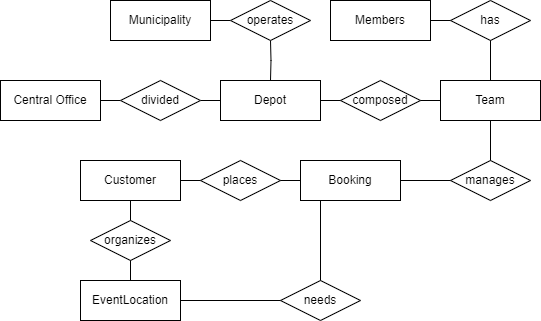
\includegraphics[width=0.7\textwidth]{./rsc/er-skeleton-schema.png}
    \caption{Conceptual skeleton schema of the database}
    \label{fig:er-skeleton-schema}
\end{figure}

\begin{figure}[H]
    \centering
    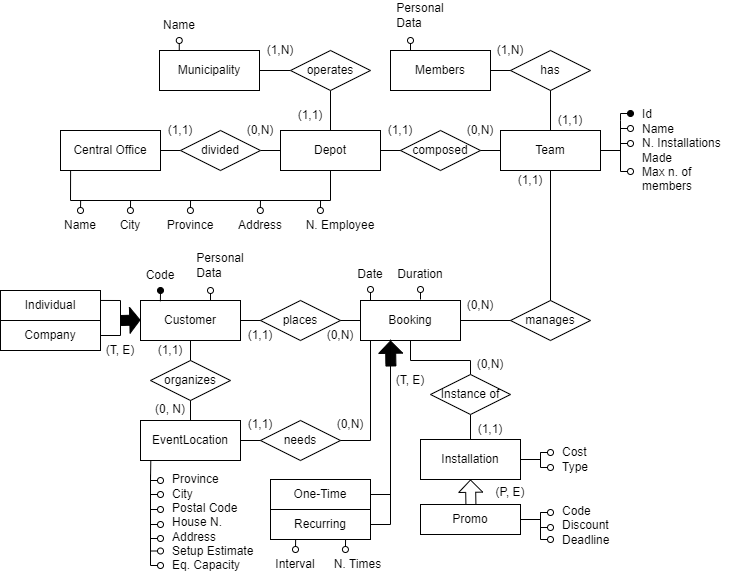
\includegraphics[width=0.7\textwidth]{./rsc/er-schema.png}
    \caption{Conceptual ER schema of the database}
    \label{fig:er-schema}
\end{figure}

\subsection{Business Rules}

\begin{enumerate}
    \item The number of employees in each depot and central office is automatically calculated as the sum of the members of all teams in that depot or central office respectively.
    \item The number of installations made by each team is automatically calculated as the number of bookings handled by that team.
    \item Each team must have a number of members less than or equal to the maximum number of members allowed for that team.
    \item Each event location setup estimate is automatically calculated as the sum of the setup times of all bookings handled at that location.
    \item Each booking can be placed only by the customer who organized the event location for which the booking is made.
\end{enumerate}